\chapter{Anexo del Proyecto Integrador}
\label{anexoPI}

\section*{Solicitud de Aprobación de Tema}
\addcontentsline{toc}{section}{Solicitud de Aprobación de Tema}
\vspace{0.5cm}

\section*{OBJETIVO GENERAL}
El presente proyecto surge ante la necesidad de contar con soluciones tecnológicas aplicadas a la agricultura urbana, un campo aún poco desarrollado en el medio local y de creciente importancia frente al aumento de la urbanización y la limitación de recursos. En este contexto, se plantea desarrollar e implementar un prototipo de granja urbana vertical inteligente, aplicando principios de la Industria 4.0, para el monitoreo y control de variables críticas de cultivo en entornos urbanos, con el fin de optimizar el uso de agua, energía y espacio, contribuyendo a la seguridad alimentaria y a la sostenibilidad ambiental.\\
A su vez, es importante remarcar que este PI es parte del proyecto del LIADE "Granjas inteligentes para ciudades inteligentes y sostenibles. Desarrollos de la Industria 4.0 para la gestión de la Agricultura Urbana y Periurbana (AUP) sostenible de ciudades inteligentes", dirigido por Oscar Vanella, para cumplir el objetivo correspondiente al año 2025 de implementación y puesta a punto de un prototipo.

\section*{OBJETIVOS ESPECÍFICOS}
\begin{enumerate}
  \item Analizar y justificar la selección de cultivos representativos a utilizar en el prototipo.
  \item Seleccionar el dispositivo electrónico adecuado para el procesamiento y gestión de datos.
  \item Diseñar la estructura física modular de tres niveles (0,5m$^2$ cada uno).
  \item Seleccionar e instalar sensores ambientales y de sustrato (temperatura, humedad relativa, humedad del suelo, luz).
  \item Implementar los sistemas de iluminación, riego, ventilación y protección frente a factores ambientales.
  \item Desarrollar la lógica de control en microcontrolador para la gestión integral del sistema.
  \item Construir e integrar el prototipo completo con sus subsistemas.
  \item Realizar pruebas de funcionamiento con diferentes cultivos en condiciones controladas.
  \item Adquirir y registrar datos de operación.
  \item Evaluar la eficiencia hídrica, energética y la estabilidad microclimática alcanzada, generando conclusiones sobre la viabilidad del sistema.
\end{enumerate}

\section*{ANTECEDENTES DE PROYECTOS SIMILARES}
En Argentina existen algunos proyectos y productos vinculados a la agricultura vertical, aunque su desarrollo aún es incipiente en comparación con otros países. La principal diferencia respecto de nuestra propuesta radica en el costo, sustrato y la versatilidad del prototipo, mientras que los sistemas disponibles suelen estar orientados a un público específico (como productores agrícolas o cultivos determinados, por ejemplo viñedos en Mendoza que han utilizado esta tecnología), el presente proyecto busca implementar una solución más accesible, adaptable y de bajo costo, que pueda ser utilizada por cualquier persona en entornos urbanos, sin necesidad de contar con conocimientos técnicos avanzados. De esta manera, se pretende acercar la agricultura inteligente a usuarios comunes y fomentar su integración en la vida cotidiana.

\vspace{0.3cm}
\noindent\textbf{Proyectos relacionados:}\\
\noindent\textit{Proyecto Integrador:}
\begin{itemize}
  \item MIGLIORE, EMILIANO. DISEÑO E IMPLEMENTACIÓN DE UN SISTEMA DE CONTROL PARA UN MÓDULO DE AGRICULTURA VERTICAL. Año 2024.
  \item IRAZUZTA, NICOLAS. MONITOREO DE INVERNADERO HIDROPONICO, MEDIANTE IoT. Año 2023.
\end{itemize}

\noindent\textit{Práctica Profesional Supervisada:}
\begin{itemize}
  \item Pieckenstainer, Mateo. Actividades realizadas en la Práctica Profesional Supervisada desarrollada en el L.I.A.D.E (Laboratorio de Investigación Aplicada y Desarrollo) relacionada con la investigación y desarrollo de granjas urbanas inteligentes.
\end{itemize}

\begin{figure}[H]
    \centering
    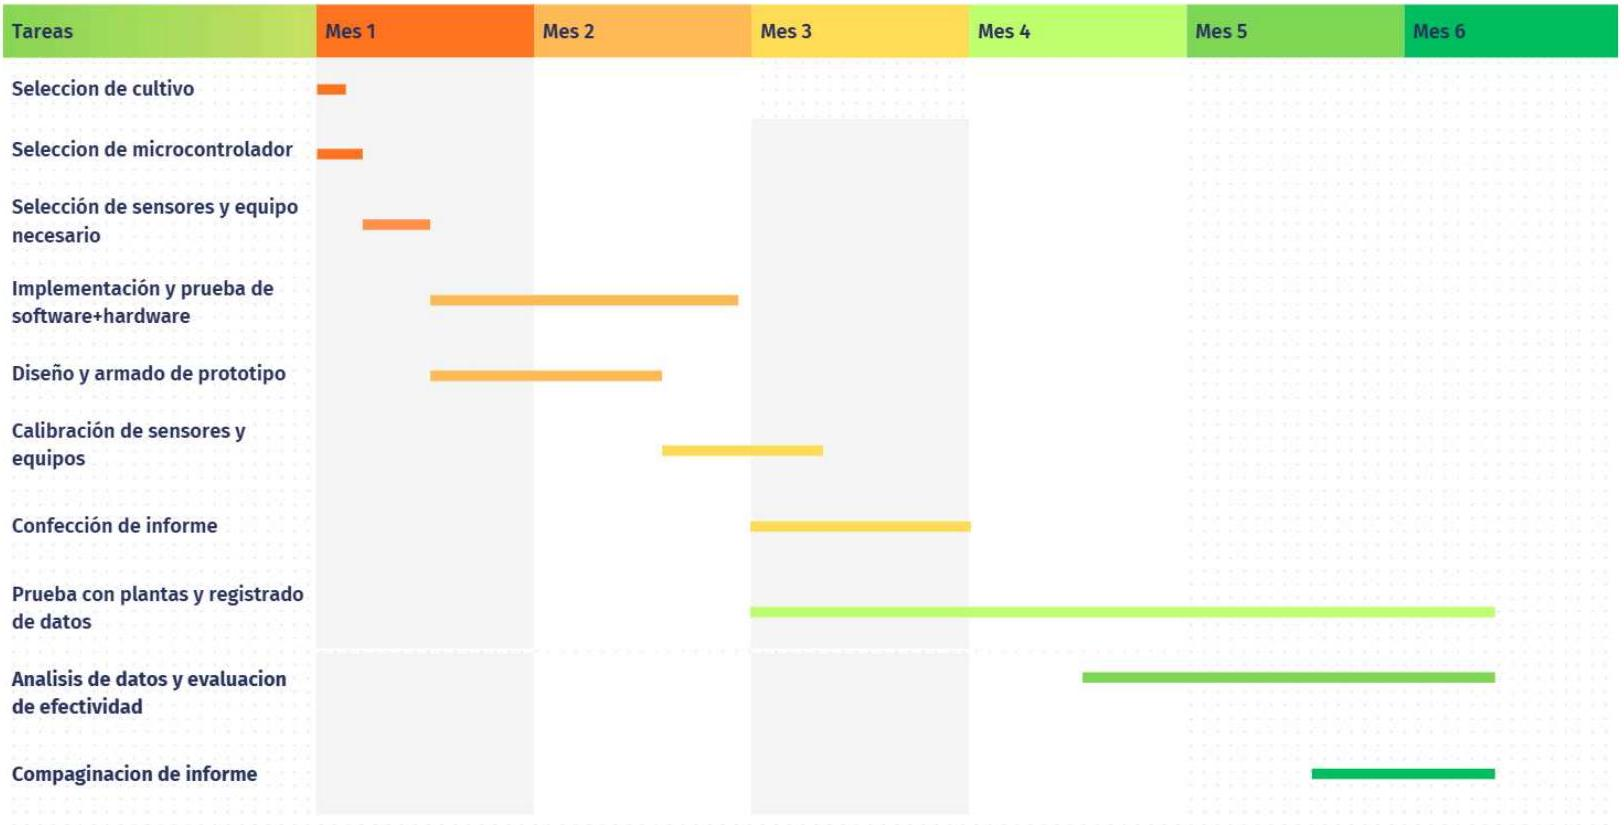
\includegraphics[height=10cm, width=\textwidth, keepaspectratio]{Imagenes/SAT1.jpg}
    \caption{DURACIÓN Y FASES DE LAS TAREAS PREVISTAS}
\end{figure}

\section*{METODOLOGÍA}
\noindent\textbf{LUGAR PREVISTO DE REALIZACIÓN:} LIADE

\vspace{0.3cm}
\noindent\textbf{REQUERIMIENTOS DE INSTRUMENTAL Y EQUIPOS:}
\begin{itemize}
  \item Microcontrolador
  \item Sensores y equipamientos (iluminación full espectro, mangueras, bombas de agua, etc.)
  \item Materiales para estructura modular
  \item Instrumentos de medición
  \item Herramientas varias
\end{itemize}

\noindent\textbf{INVERSIÓN DE DINERO ESTIMADO:} Aproximadamente USD 400-500 (a cargo del LIADE)\\
\textbf{APOYO ECONÓMICO EXTERNO A LA FACULTAD:} No.

\vspace{0.5cm}
\noindent Recibido Cátedra PI \underline{\hspace{4cm}}

\noindent Córdoba, \underline{\hspace{4cm}}

\vspace{1cm}

% --- INICIO DEL ANEXO DETALLADO ---

\section*{ANEXO: DESCRIPCIÓN DETALLADA DEL PROYECTO}

El presente proyecto tiene como finalidad el diseño e implementación de un prototipo de granja urbana inteligente a escala reducida, que funcione como plataforma experimental para el estudio y validación de sistemas de monitoreo y control aplicados a la Agricultura Urbana y Periurbana. La propuesta se enmarca en el contexto de la Agricultura 4.0, donde la incorporación de sensores, automatización y tecnologías de la información permite optimizar recursos y garantizar la sostenibilidad en la producción de alimentos en entornos urbanos. La iniciativa busca responder a una problemática actual: el crecimiento de la población y la urbanización que, junto con la reducción del suelo cultivable, impulsan la necesidad de nuevas soluciones que permitan producir alimentos de manera eficiente, segura y sustentable dentro de las ciudades.

El prototipo a desarrollar consistirá en una estructura modular de cultivo vertical, diseñada para albergar varios niveles apilados en los que se dispongan plantas representativas elegidas durante la fase de diseño. La elección de las especies se realizará considerando criterios de pertinencia regional, facilidad de manejo, rusticidad y diferentes requerimientos lumínicos e hídricos, de modo que el sistema pueda ser evaluado en condiciones diversas. La estructura deberá permitir un montaje firme, accesible y seguro, con dimensiones compatibles con un entorno de laboratorio, y será diseñada de manera que pueda ser escalable y replicable en el futuro.

Para garantizar el desarrollo adecuado de los cultivos, el sistema integrará distintos subsistemas. En primer lugar, se dispondrá de un subsistema de sensado que permita medir variables ambientales y del sustrato críticas para el crecimiento de las plantas. Entre estas variables se incluyen la temperatura y la humedad relativa del aire, la humedad del sustrato y la intensidad lumínica recibida por los cultivos. Los sensores seleccionados serán definidos durante el proceso de diseño, buscando siempre un equilibrio entre precisión, costo y facilidad de integración. La información recolectada por estos sensores será procesada por un microcontrolador, que actuará como unidad central de control, ejecutando las decisiones necesarias para mantener las condiciones dentro de rangos adecuados y proporcionando al usuario información sobre dichas condiciones. 

\begin{figure}[H]
    \centering
    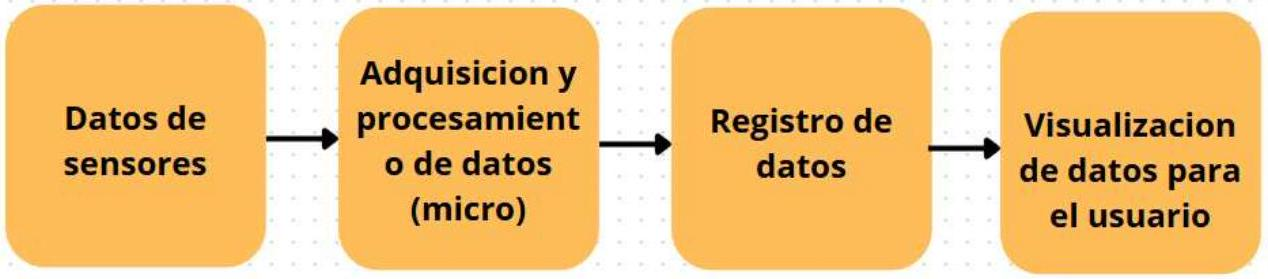
\includegraphics[height=10cm, width=\textwidth, keepaspectratio]{Imagenes/SAT2.jpg}
    \caption{}
\end{figure}

El subsistema de riego será diseñado de manera que garantice un suministro uniforme y eficiente de agua, evitando tanto el déficit como el exceso de humedad. Se analizarán alternativas como el riego por goteo o microaspersión, que se encuentran entre las más utilizadas en sistemas urbanos de pequeña escala. Además, se evaluará la posibilidad de implementar un mecanismo de recirculación, mediante el cual el agua excedente pueda ser recolectada, filtrada y reutilizada, contribuyendo así a la eficiencia hídrica del sistema. La activación de este subsistema se llevará a cabo automáticamente según la información provista por los sensores de humedad de sustrato.

En paralelo, el sistema contará con un subsistema de iluminación artificial que simule el aporte lumínico necesario para el crecimiento vegetal. Se prevé el uso de tecnologías que ofrezcan un espectro adecuado para la fotosíntesis, como sistemas de iluminación LED, cuyo dimensionamiento y disposición serán definidos durante el diseño. El encendido, apagado y regulación de las luces se realizará desde el microcontrolador, permitiendo programar fotoperiodos específicos y garantizar que cada nivel de cultivo reciba la cantidad adecuada de radiación.

Dado que el ambiente de cultivo en estructuras verticales tiende a acumular humedad y calor, se integrará un subsistema de ventilación que permita la circulación de aire y la homogeneización de las condiciones internas. Para ello, se considerará la instalación de ventiladores de baja potencia, estratégicamente distribuidos para favorecer la renovación de aire y reducir riesgos asociados a hongos y enfermedades. Este subsistema también será controlado por la unidad central, que lo activará según los valores de temperatura y humedad registrados.

La unidad de control central, basada en un microcontrolador, será el eje del prototipo. Su función principal será integrar la información proveniente de los sensores y accionar los diferentes subsistemas: riego, iluminación y ventilación. Además, se analizará la inclusión de un sistema de almacenamiento de datos y una interfaz de usuario, que podría consistir en la transmisión de datos a un dispositivo externo, lo que permitiría registrar información, visualizarla y analizar tendencias. De esta manera, se obtendrá un registro continuo que permitirá evaluar el desempeño del sistema y la respuesta de los cultivos.

\begin{figure}[H]
    \centering
    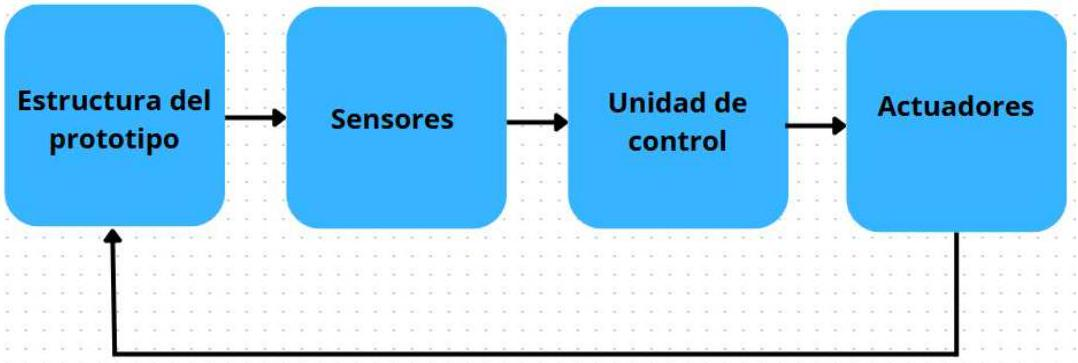
\includegraphics[height=10cm, width=\textwidth, keepaspectratio]{Imagenes/SAT3.jpg}
    \caption{}
\end{figure}

La metodología de trabajo se organizará en distintas fases. En una primera etapa se realizará la selección de cultivos representativos y de los componentes tecnológicos a utilizar, incluyendo sensores, actuadores y dispositivos de control. Posteriormente se llevará a cabo el diseño de la estructura física, la cual será construida con materiales resistentes y accesibles, garantizando estabilidad y facilidad de montaje. Una vez definida la estructura, se procederá a la construcción y montaje de los subsistemas de riego, iluminación y ventilación, junto con la instalación del microcontrolador y los sensores. En la siguiente fase se integrarán hardware y software, desarrollando la lógica de control y calibrando los sensores en condiciones de laboratorio. Finalmente, se llevarán a cabo pruebas experimentales con los cultivos seleccionados, durante las cuales se registrarán datos útiles. Estos datos serán luego analizados para evaluar la eficiencia del sistema, la estabilidad del microclima y la viabilidad del prototipo como modelo de granja urbana inteligente.

\begin{figure}[H]
    \centering
    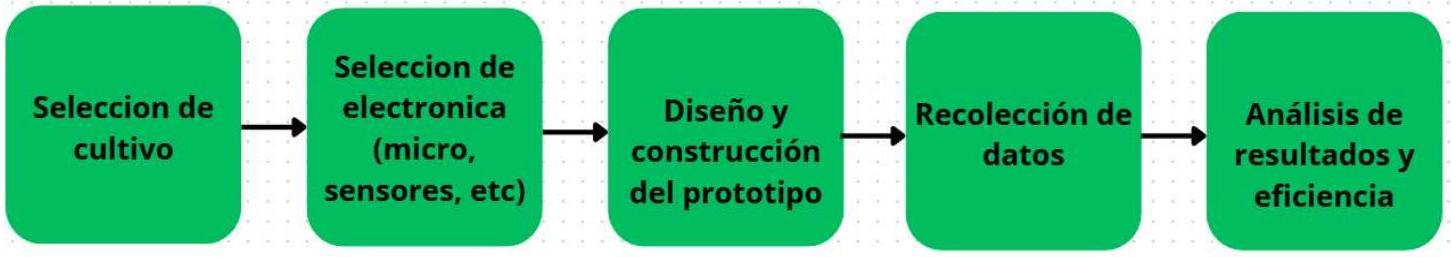
\includegraphics[height=10cm, width=\textwidth, keepaspectratio]{Imagenes/SAT4.jpg}
    \caption{}
\end{figure}

Asimismo, se prevé la posibilidad de futura integración con desarrollos complementarios de redes IoT, con el propósito de ampliar las capacidades de monitoreo remoto sin alterar el alcance central de este trabajo.

El resultado esperado es la validación de un prototipo funcional de granja urbana vertical, capaz de demostrar que la integración de monitoreo y control automatizado permite mejorar la eficiencia en el uso de recursos y garantizar un entorno de cultivo más estable y predecible. Además, se espera generar métricas concretas sobre consumo de agua y energía, así como sobre la respuesta de los cultivos en condiciones controladas. Este conocimiento podrá servir de base para desarrollos futuros, con miras a la escalabilidad del sistema y a su aplicación práctica en distintos entornos urbanos.

\section*{REFERENCIAS BIBLIOGRÁFICAS Y DE SOFTWARE}
% Asegurate de tener \usepackage{hyperref} o \usepackage{url} en tu preámbulo
\begin{itemize}
    \item \url{https://extension.umd.edu/resource/6-pasos-basicos-para-empezar-o-plantar-un-huerto-vegetal/}
    \item \url{https://www.argentina.gob.ar/produccion/planargentina40/industria-4-0}
    \item \url{https://blog.oxfamintermon.org/como-hacer-un-huerto-en-casa-con-poco-espacio/}
    \item \url{https://agrospray.com.ar/blog/agricultura-vertical/}
\end{itemize}

\section*{Informes mensuales}
\addcontentsline{toc}{section}{Informes mensuales}

Aquí van los informes mensuales ordenados por fecha. Debe retirarse todo dato personal y firmas.